\documentclass[%
aip,
amsmath,amssymb,
%aps,
%twocolumn,
%preprint,%
reprint,%
unsortedaddress,
nofootinbib
%author-year,%
%author-numerical,%
]{revtex4-2}

\usepackage{nicefrac,siunitx}
\usepackage{color}
\usepackage{tikz,tikzscale}\usetikzlibrary{shapes}
\usepackage{enumitem}
\usepackage{hyperref,cleveref}
%\usepackage{emoji}

\usepackage[local]{gitinfo2}
\usepackage{xargs,ifthen}

\usepackage[nolist]{acronym}

% Editing
\usepackage[
	final
]{changes}
\presetkeys{todonotes}{
	inline,
	disable
}{}
\usepackage{draftwatermark}
\SetWatermarkText{DRAFT}
\SetWatermarkScale{1}
\SetWatermarkColor[gray]{0.75}

\newcommandx{\dec}[2][1={},2={}]{_{#1}
		\ifthenelse{\equal{#2}{}}{}{^{#2}}
}
\newcommandx{\Node}[2][1={},2={}]{N\dec[#1][#2]}
\newcommandx{\Root}[2][1={},2={}]{R\dec[#1][#2]}
\newcommandx{\Arg}[2][1={},2={}]{A\dec[#1][#2]}

\newcommandx{\Children}[2][1={},2={}]{\mathcal{C}\dec[#1][#2]}
\newcommandx{\Siblings}[2][1={},2={}]{\mathcal{S}\dec[#1][#2]}

\newcommandx{\wgt}[2][1={},2={}]{w\dec[#1][#2]}
\newcommandx{\imp}[3][1={},2={},3={}]{I\dec[\ifthenelse{\equal{#3}{}}{}{#3,}#1][#2]}
\newcommandx{\impOwn}[3][1={},2={},3={}]{I'\dec[\ifthenelse{\equal{#3}{}}{}{#3,}#1][#2]}
\newcommandx{\liq}[2][1={},2={}]{n^{\T}\dec[#1][#2]}

\newcommandx{\mixing}[2][1={},2={}]{\gamma\dec[#1][#2]}

\newcommandx{\supportive}[2][1={},2={}]{\sigma\dec[#1][#2]}


\newcommand{\tot}{\text{total}}
\newcommand{\sib}{\text{siblings}}

\newcommand{\T}{\text{T}}
\newcommand{\Y}{\text{Y}}
\newcommand{\N}{\text{N}}

\begin{document}
\title{ArborVote -- Deliberative Decision-Making using Argument Trees \deleted[comment={Discuss multiple ways of determining the impact}]{and Rating Markets}}
\author{Michael A. Heuer}
%\email[Email:]{}
\date{\today, Version: \gitDescribe}

\begin{abstract}
Decision-making based on arguments is unpopular because of the bureaucratic overhead connected to it. 
The centralized online platform \href{https://www.kialo.com/}{www.kialo.com} overcomes this issue and 
	keeps debates rational, 
	presents them in a structured and transparent way, and, thus,
	allows for fast on-boarding of participants.
Participants create a tree of pro and con arguments and can express preference by rating their impact. 
However, the platform cannot be used as a governance tool because it lacks resilience against manipulation and Sybil attacks.
This gap can be filled with blockchain technology by
	providing a tamper-proof voting infrastructure,
	using decentralized digital identities, and
	creating economic incentives for participation.
This is the motivation behind ArborVote, a voting module for deliberative decision-making using argument trees that can be integrated into existing \aclp{DAPP} and \aclp{DAO}.
\end{abstract}

\keywords{Governance, Voting, Deliberative Democracy, Decision Making, Argument Trees, \acsp{DAO}}

\maketitle

% No indentation
\setlength{\parindent}{0cm}
\setlength{\parskip}{0.4em plus0.1em minus0.1em}

\begin{acronym}
	\acro{AMM}{automated market maker}
	\acro{CPMM}{constant product market maker}
	\acro{PM}{prediction market}
	\acro{RM}{rating market}
	\acro{DAPP}{decentralized application}
	\acro{DAO}{decentralized autonomous organization}
	\acro{DLT}{distributed ledger technology}
	\acroplural{DLT}[DLTs]{distributed ledger technologies}
	\acro{DAG}{directed acyclic graph}
	\acro{MACI}{minimal anti-collusion infrastructure}
	\acro{L2}{layer 2}
\end{acronym}

%\tableofcontents

\todo{
	Applications: use in DAOs but also Courts (DApps)
}

%%%%%%%%%%%%%%%%%%%%%%%%%%%%%%%%%%%%%%%%%%%%%%%%%%%%%%%%%%%%%%%%%%%%%%%%%%%%%%%%
\section{Introduction}
%%%%%%%%%%%%%%%%%%%%%%%%%%%%%%%%%%%%%%%%%%%%%%%%%%%%%%%%%%%%%%%%%%%%%%%%%%%%%%%%

% Blockchain & Smart Contracts
Since the inception of the Ethereum blockchain in 2014\cite{Wood2014}, 
the decentralized and permissionless execution of arbitrary programs 
called smart contracts has become possible. 
This technology enables new forms of decentralized collaboration 
and governance and billions worth of dollars are currently managed by \acp{DAO}.

% Blockchain Voting
Blockchains or, more generally speaking, \acp{DLT}, provide a tamper-proof voting infrastructure
and reduce the bureaucratic and organizational overhead of a vote significantly.
Recently, digital identities, such as \href{https://www.brightid.org/}{BrightID}, \href{https://www.proofofhumanity.id/}{Proof of humanity}, and \href{https://www.idena.io/}{Idena},  became available on the blockchain and can ensure that only humans participate and have fair voting shares.
With the recent advent of scaleability solutions\todo{add citation to \ac{L2}, optimisimn, arbitrum, zk-sync/porter, starknet},
more complicated governance structures are now becoming possible.

% Status Quo of Voting Protocols
So far, simple ballot protocols, such as 
single-choice, 
multiple-choice, 
weighted,
and quadratic voting, 
have been used.
% Gap
However, 
decision options might have far-reaching consequences that the voter is not aware of, misinformed about, 
%% Cognitive Load
or have so many aspects making them difficult to structure and weight because the voter is overwhelmed by the information.
%% Voter subjectivity
Lastly, the voters have no incentive to consider other perspectives and leave their social bubble. 
%% Lacking Resilience against Misinformation and Populism
In this situation and due to lack of time and attention, voters tend to make gut decisions being based on trust in leading figures.
Populists can take advantage of the situation by influencing voters with misinformation strategies and emotionalization of the debate.

% Deliberative Democracy
Instead of expressing preferences for specific decisions options directly, 
deliberative democracy tries to find consensus on the best decision option based on deliberation, reasoning, and weighting of the individual aspects of the decision spectrum in a debate.
This way, the reasoning behind the different decision options becomes transparent to the participants and the public.
% Debates
Traditional debates are often held linearly---either in a podium discussion or in a forum.
Following such a debate passively is cognitively challenging and requires a large time investment
to present, structure, and weight different arguments.
This is even more pronounced when actively participating in a debate.
%% Complexity
The more aspects play into a decision, the more complex the debate connected to it becomes.
As a result, the number of participants in a debate is very limited and the process cannot scale.\todo{}
%% Consensus
In the best case, the debaters find consensus on which decision options they want to choose.
This is ideal and highly legitimizes the decision.
%% Fallback to Majority Voting
However, often not all participants agree and no consensus is found.
In this case, participants have to resort to a simple majority vote.
% Improvements by Digitialization
These circumstances can be improved by digitalization of the processes through
\begin{itemize}[noitemsep]
	\item structuring the debate to provide quick on-boarding of participants,
	\item formalizing the deliberation and argument weighting process, and
	\item determining the argument impacts and incentivizing participation. \todo{Impact is unclear at this point}
\end{itemize}

% Legitimization
This legitimizes the decision process by design because the reasoning and weighting behind the different arguments becomes transparent.
If voting is conducted publicly, which is still the common practice in \acp{DAO} today, 
people can also be held accountable for misjudgment.

% Why Blockchain
Since digital debating platforms (such as \href{https://www.kialo.com/}{kialo}) do exist online,
the question might arise why \acp{DLT} are needed to construct and execute a decision from a debate.
%
Three requirements favor the usage of \acp{DLT}.
% Tamper-Proof Infrastructure
First and foremost, voting processes require a tamper-proof and permissionless infrastructure that cannot be guaranteed with centralized technologies.
% Sybil protection
A second requirement is Sybil protection. 
Curated registries of unique digital identities are already available on several blockchains. 
% Incentivization
A last and optional requirement is the ability to incentivize participation.
Because the time and collective attention of the people are scarce resources,
the ability to allocate reputational or monetary rewards is useful
and especially easy to realize in the form of blockchain tokens.
To put this rather economic view in perspective:
One might see this deliberative decision-making as the decentralization of the job of politicians and consultants that are also getting paid.


\todo{
\section{Design Rationale}
}
\todo{
TODO:
The main idea for voting is to influence the outcome of the decision, taking into account one's own benefit and perspective.
As discussed earlier, this might not result in the best decision outcome for the commons.

Reversing this and incentivizig voters to consider different perspectives is not easy. 

This can only be achieved if deliberating and weighting of the arguments is more favorable than steering the decision outcome towards one's own interests.
}

\deleted{
\subsection{Trust assumptions}
%\subsection{Blockchain Infrastructure}
The voting module described here is designed to run on a permissionless blockchain infrastructure---a distributed ledger capable of decentralized execution of smart contracts  and storage of their outcomes
such as the aforementioned Ethereum blockchain\cite{Wood2014}.

The system is intended to be trustless---in other words: it can be used in a setting in which people don't know and trust each other. 
}

\section{Structuring Debates in Argument Graphs}\label{sec:Structure}
The reasoning behind decision-making is rarely linear. 
Starting from a proposal constituting the root of a debate, 
numerous, sometimes interdependent arguments are branching off. 
This results in a tree structure as depicted in \cref{fig:Tree},
where arguments constitute the tree nodes.

\begin{figure}
	\resizebox{0.95\linewidth}{!}{
		\includegraphics{Graphics/Tree.tikz}
	}
	\caption{
		Visualization of a debate as an argument tree with 
		the root node $\Root$ (dashed) and 
		argument nodes $\Arg$ (solid)
		numbered by their order of creation.
		Nodes have an impact $\imp$ and a weight $\wgt$ relative to their siblings 
		and can support or oppose their associated parent as indicated by green and red links, respectively.
	}
	\label{fig:Tree}
\end{figure}

In contrast to other voting algorithms, ArborVote incorporates this tree of arguments into the voting process,
which is briefly outlined in the following.

Here, the creator of the debate posts a proposal forming the root $\Root$ of the debate tree.
This root node is expressed as a statement, e.g., 'We should execute process A.'
that can be supported or opposed by the debate participants.
To facilitate multiple decision options, 
a forest containing
multiple trees can be constructed---all of them having their own root statement, 
e.g., 'We should execute process B.'.

Next, debate participants can create arguments $\Arg$ below the root node
but also other argument nodes that are either supporting (pro arguments) or opposing (con arguments) the their parent node they are referring to.
%
To identify each node $\Node$ in the tree, the notation $\Node[i][p]$ is used, 
where $i$ and $p$ are unique identifiers of the argument itself and its parent, respectively.
For convenience, we define the set containing the identifiers of all children and siblings of a node $\Node[i][p]$ by $\Children[i]$ and $\Siblings[i]\equiv\Children[p]$


ArborVote aims to provide an incentive structure 
to motivate actors participating constructively in the debate and 
to identify and rate the impact of valuable arguments.
To maintain a clear structure and overview, arguments have to be curated.
Moreover, because constructive participation should be rewarded and malicious, destructive behavior should be penalized, 
creators have to put something at stake
and their ownership of an argument must be clearly assigned.

In the following, the different phases and stakeholder roles are introduced.

\section{Phases, Stakeholders, and Stakes of the Debate}\label{sec:DebatingProcess}
\todo{Motivate formalization before?}

The decision-making process in ArborVote consists of three phases:
\begin{enumerate}[noitemsep]
	\item editing
	\item rating
	\item tallying
\end{enumerate}
in which participants can occupy one or multiple of the roles listed below
\begin{itemize}[noitemsep]
	\item debaters
	\item curators
	\item jurors
	\item voters
\end{itemize}
In the following, these roles are briefly presented.
Debaters author arguments and add them to the debate tree.
Curators can flag and propose edits to the content that authors can accept or reject.
In the latter case, a dispute is raised that is resolved by jurors in a digital court.
Lastly, voters can invest debate tokens to rate the impact of nodes in the debate tree.
To maintain neutrality, jurors are excluded from the other roles.

% Debate Tokens
\todo{Move elsewhere}
In this system, 
each participant has a predefined amount of debate tokens $\T$ that can only be spend within the debate.
These are either distributed equally among the participants or based on the reputation in the \ac{DAO}.
%
Participants can spend the debate tokens 
to create, curate, and rate arguments.
%
The system rewards participants behaving deliberate- and constructively in the debate, 
which is described in\replaced{the following}{ \cref{sec:Incentives}}.

\subsection{Editing Phase}\label{sec:EditingPhase}
Because the goal is to reward constructive participation in the debate, 
the ownership of the arguments is clearly assigned.
Accordingly, debaters own the arguments they authored themselves.
To allow others to consider the argument and to prevent duplicates, it is immediately visualized in the tree.

Within a predefined grace-period, an argument owner can edit the argument or create arguments below, 
whereas other participants cannot.
However, other participants can suggest edits, moving, or removal of the arguments and are thus called curators.

The editing of the author includes 
\begin{itemize}[noitemsep]
	\item altering the text (without changing the meaning) % check if timestamp 
	\item moving the node (i.e, changing the parent to a different finalized node)%changing the link
	\item posting sub-nodes
	\item deleting the node
	\item accepting edits / move suggestions from curators
\end{itemize}
After the grace period, the argument becomes finalized.
This finalization allows other debaters to support or oppose the finalized argument with more arguments.


\subsubsection*{Ownership, Curation, and Dispute Resolution}
%Despite suggesting edits or removal of arguments,
Disputes about argument ownership might arise, 
if duplicates or very similar statements are present in different parts of the tree.
Curators can flag nodes containing 
plagiarism, 
spam, or 
offensive content such as hate-speech or sexism. 
In order to raise a dispute, 
curators have to lock up a deposit, 
i.e, tokens that have monetary value and are not debate tokens. 
If the argument author agrees with the accusation, he/she can remove the argument \replaced{and pay only a small}{without any} penalty of the deposited debate tokens \added{to the curator}. 
If not, the author has to match the deposit and the dispute is escalated to a digital court such as \href{https://kleros.io/}{Kleros Court}\cite{Lesaege2019,Lesaege2021} or \href{https://anj.aragon.org/}{Aragon Court}\cite{Cuende2019}.

Depending on the court decision, the node either remains in the tree or is deleted.
As a result, either the creator or curator loses the deposit, which is then split between the opposing side and the jurors. 
\todo{What happens to the debate tokens? Curator gets them but cannot spend them - used for reputation rewards in the end}


\subsection{Rating Phase}\label{sec:RatingPhase} % Voting Phase
After the editing phase ended and the argument tree is completely finalized,
the debate enters the rating phase---the actual voting process.

% challenge
% Design rationale
\highlight{The key challenge} here is to incentivize the participants to 
rate the impact $\imp$ of an argument and to decouple it from the individual outcome preference. 
In simple terms, the goal is to eliminate tactical voting.
Voting solely with the goal to influence the decision should be an unprofitable strategy.

% Rating markets
This design rationale can be achieved by employing a market mechanism---we call this a \ac{RM}.
%This impact is determined separately for each argument via a market mechanism that we call \ac{RM}.
A \ac{RM} is a slightly modified \ac{PM} such as the \href{https://omen.eth.link/}{Omen \ac{PM}}\cite{Omen2020} and also uses an \ac{AMM}\cite{Zhang2018} for liquidity provision.
Participants can spend their debate tokens to invest in approval or disapproval shares $\Y$ and $\N$
\deleted{being minted at the current market ratio}.
These participants are called voters.

% Impact signal
The amount of approval and disapproval shares $n^\Y$ and $n^\N$ in the \ac{AMM}
signals the impact as a scalar value between $0$ and $1$
\begin{equation}
	\imp = 1-\frac{n^\Y}{n^\Y+n^\N},
\end{equation}
where the second term corresponds to the relative share of $\Y$ tokens available at the market.
Accordingly, the less approval shares $n^\Y$ are available at the market, the higher the impact $\imp$.


% PM contrast
In contrast to a conventional \ac{PM} where all shares except that of the correctly predicted outcome (determined by an oracle) are invalidated after the market close,
all shares maintain their last value and are redeemed for debate tokens. 
\todo{How to prevent unwanted dynamics shortly before the market close?}
% Arbitrage
Accordingly, voters who buy approval or disapproval shares of under- or overrated arguments that turn out to be rated higher or lower at the market close, respectively, make a profit in debate tokens.

% Liquidity provision by the author
The liquidity of the \ac{AMM} is provided by the author of the argument who has to deposit debate tokens at the point of the creation of the argument.
Moreover, the author determines the initial amount of the approval and disapproval shares $n^\Y$ and $n^\N$ minted from the debate tokens at the market start
and therefore the initial impact $\imp$.
If the argument creator does not specify a ratio, 
the amount of approval and disapproval tokens is set with $n^\Y=n^\N=\nicefrac{1}{2}\,n^\T$. 
% Fees and Permanant Loss
As in every \ac{AMM}, liquidity providers (here the author \todo{and editors of the argument})
earn fees of traders (here voters)
and 
take the risk of suffering permanent loss, if the market diverges from the initial value.
This incentivizes authors to evaluated their own arguments impact critically 
\deleted[comment={Should the final earning/loss be related to $\imp$ or $\impOwn$}]{and to take also related child arguments into account}
to minimize permanent loss. 
% Initial impact
To disincentivizes debaters to create bad arguments and earn on the fees,
the initial ratio is limited to $[\nicefrac{1}{2},1)$ (or even a more conservative lower limit $>\nicefrac{1}{2}$).
The value $\imp=1$ is excluded because otherwise, the constant product $\Y\times \N = 0$.
% RM details
The details of the rating market mechanics are discussed in detail in \cref{sec:RatingMarkets}

% Design Rational
In summary, these mechanics incentivize, both, the debaters and voters, to consider and multiple arguments and perspectives.
 
Debating and voting solely with the goal to influence the decision is an unprofitable \deleted{long-term} strategy resulting
as the actors end up with \highlight[comment={How to proof this?}]{less vote tokens than the average participant.}
\todo{Discuss in more detail.}

% Tallying
In the subsequent tallying phase,
the impact value $\imp$ determined by the markets is tallied up,
which is described in the following section.


\subsection{Tallying Phase}\label{sec:TallyingPhase}
In the tallying phase, the impact of the different nodes is accumulated and weighted.
We define the weight of a node $\Node[i]$ by
\begin{equation}
	\wgt[i] = \frac{\liq[i]}{\liq[i]+\sum_{j\in \Siblings[i]}\liq[j]}
\end{equation}
as the amount of debate tokens spent $\liq[i]$ relative to its siblings $\Siblings[i]$.

to the total number of deposited debate tokens of its siblings.
This allows for expressing the impact of a node $\Node[i]$ by
\begin{equation}\label{eq:Impact}
	\imp[i] = 
	\max
	\left[\vphantom{\sum}\right.
	0
	\,,\,
	\underbrace{(1-\mixing[i])\cdot\impOwn[i]}_{\text{own}} 
	+
	\underbrace{\mixing[i]\cdot\imp[i][\Children]}_{\text{children}}
\left.\vphantom{\sum}\right],
\end{equation}
as two terms scaled with a mixing parameter $\mixing[i]$.
The $\max$ operator ensures that the overall impact value cannot become negative.

The first term contains the nodes own impact $\impOwn[i]$ being determined directly from the associated \ac{RM}.
The second term contains the weight-averaged impact of all children nodes 
\begin{equation}
	\imp[i][\Children] = \sum_{j\in \Children[i]} \supportive[j]%[i] 
	\imp[j]\,\wgt[j].
\end{equation}
with the pre-factor
\begin{equation}
	\supportive[j]%[i]
	=
	\begin{cases}
		+1 & \text{if node $j$ is supporting}\\
		-1 & \text{if node $j$ is opposing}
	\end{cases},
\end{equation}
resulting in the subtraction of impact, if the associated node opposes its parent.
% Mixing
Both terms are scaled with the mixing parameter $\mixing$.
The higher the value of $\mixing$, the more influence the children nodes have on $\imp[i]$.
Because the influence of a single node on the decision outcome decreases with increasing distance from the tree root, 
it becomes less attractive to add too many layers to the tree, which incentivizes keeping debates short.

Special cases arise for the different node types in the tree:
\begin{equation}
	\mixing[i] =
	\begin{cases}
		1 & \text{if $\Node[i]$ is root ($i=0$)}\\
		0 & \text{if $\Node[i]$ is leaf}\\
		k \in[\nicefrac{1}{2},1) & \text{else}
	\end{cases}
\end{equation}
% root
For the root node, the impact is solely determined from the child impacts  ($\mixing=1$).
% leaf
For a leaf node, the impact is determined solely from its own rating market ($\mixing=0$).
% all others
For all other nodes,
the ratio between the two is defined by constant $k\in[\nicefrac{1}{2},1)$ specified by the debate creator.


\todo{Add example.\\ 
For example with $k=\nicefrac{3}{4}$...
}


\todo{
\section{Incentive Structures}\label{sec:Incentives}
% Creation
\subsection{Rewards}
- debate summoner has to offer rewards (either reputation or money)
- rewards are split between participants that performed above average
}


\section{Attack Scenarios}
In the following, different attack scenarios and means for mitigation are discussed.

\subsection{Spamming Attacks}
The number of nodes that can be created is limited by the number of debate tokens and
curators can remove the spam nodes.

\subsection{Ownership Attacks}
Duplicates and plagiarism can be identified by  curators via the node's time-stamp
or ultimately decided by jurors in a court.

\subsection{Sybil-Attacks}
Curated registries such as \href{https://proofofhumanity.id/}{Proof of Humanity}
ensure that only real humans participate.


\subsection{Collusion}
Collusion (such as bribery or blackmailing) is still an open problem in decentralized governance.
However, it can be solved in the future if \href{https://ethresear.ch/t/minimal-anti-collusion-infrastructure/5413}{\ac{MACI}}\cite{Buterin2021} becomes available.
In the context of ArborVote this means that the debate participants remain secret and cannot proof to each other that they have created or voted for a certain tree node.


%%%%%%%%%%%%%%%%%%%%%%%%%%%%%%%%%%%%%%%%%%%%%%%%%%%%%%%%%%%%%%%%%%%%%%%%%%%%%%%%
\section*{Acknowledgments}
%%%%%%%%%%%%%%%%%%%%%%%%%%%%%%%%%%%%%%%%%%%%%%%%%%%%%%%%%%%%%%%%%%%%%%%%%%%%%%%%

%This work was generously supported by ETH Research Grant ETH-20 15-1 and ETH Pioneer Fellowship Grant PIO-11-14-2.

Discussions
with 
James Simbouras,
\highlight{Dan13ram},
Daniel Ospina,
Matt Prewitt, 
Manu Flores,
are gratefully acknowledged.


%%%%%%%%%%%%%%%%%%%%%%%%%%%%%%%%%%%%%%%%%%%%%%%%%%%%%%%%%%%%%%%%%%%%%%%%%%%%%%%%
\section*{Appendix}
%%%%%%%%%%%%%%%%%%%%%%%%%%%%%%%%%%%%%%%%%%%%%%%%%%%%%%%%%%%%%%%%%%%%%%%%%%%%%%%%

\subsection*{Rating Markets}\label{sec:RatingMarkets}
An \ac{AMM}, more specifically a \ac{CPMM}, is used to provide liquidity for the rating markets.
The argument creator deposits $n^\T$ debate tokens 
to mint 
$n^\Y$ approval ($\Y$) and 
$n^\N$ disapproval ($\N$) shares
%at a price ratio
%\begin{equation}
%	\label{eq:PriceRatio}
%	p = \frac{n^\Y}{n^\N}
%\end{equation}
so that
\begin{equation}
	n^\Y+n^\N = \liq.
\end{equation}
The $\Y$ and $\N$ tokens form a trading pair
whose product has to remain constant
\begin{equation}
	k = n^\Y\cdot n^\N.
\end{equation}

If a voter invests debate tokens to buy, e.g., approval shares,
both share types are minted at the \highlight{current} \ac{AMM} ratio of $n^\Y: n^\N$.
Then, the unwanted shares are sold at the \ac{AMM} for the wanted share type, 
which is the same implementation as in 
\href{https://omen.eth.link/}{Omen \acp{PM}}\cite{Omen2020}.
An example is depicted in \cref{fig:RatingMarket}.
\begin{figure*}
	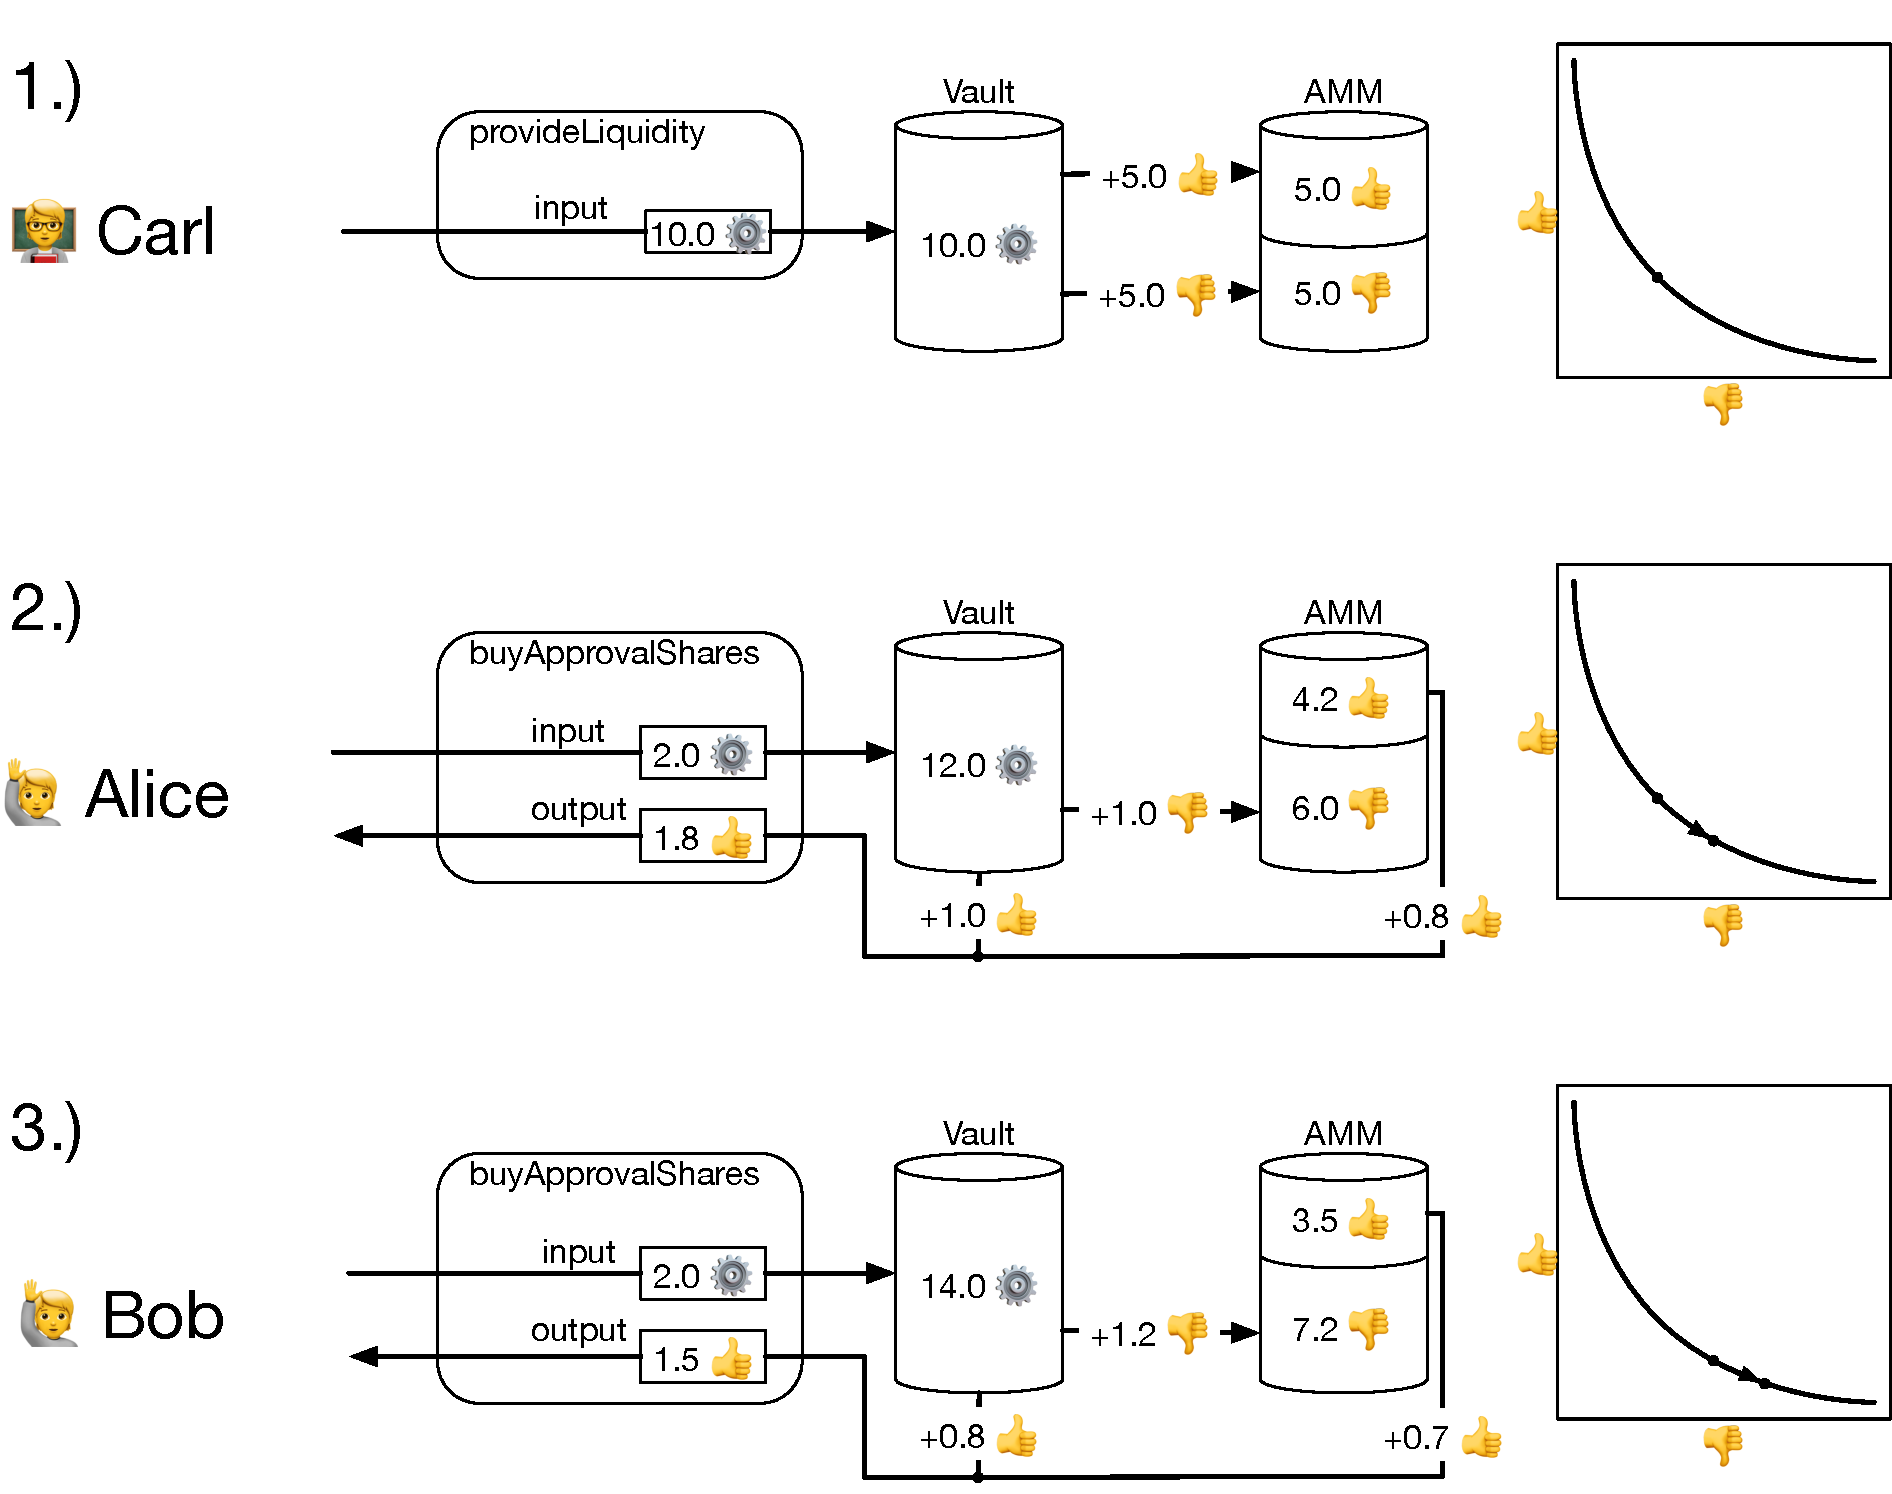
\includegraphics[width=0.75\textwidth]{Graphics/RatingMarket.pdf}
	\caption{Process flow diagram in a rating market showing
	1.) liquidity provision by the argument creator Carl with a ratio of $n^\Y:n^\N=1$
	and 
	two consecutive market trades by 
	2.) Alice and 
	3.) Bob where each of them buys approval shares for an equivalent of 2\,\T{} on the underlying \ac{CPMM}.
	After the market close, 
	Alice and Bob redeem their approval shares \Y{} for \num[round-mode=places,round-precision=1]{2.534597515403166}
	and
	\num[round-mode=places,round-precision=1]{2.0801261686545804}
	debate tokens \T{}, thus generating profit.
	Carl redeems his \Y{} and \N{} shares for
	$\num[round-mode=places,round-precision=1]{4.813525792017222}\,\T
	+\num[round-mode=places,round-precision=1]{4.571750523925031}\,\T
	=\num[round-mode=places,round-precision=1]{9.3852763159}\,\T$, thus suffering a loss.
}
	\label{fig:RatingMarket}
\end{figure*}


%%%%%%%%%%%%%%%%%%%%%%%%%%%%%%%%%%%%%%%%%%%%%%%%%%%%%%%%%%%%%%%%%%%%%%%%%%%%%%%%
%\section*{References}
%%%%%%%%%%%%%%%%%%%%%%%%%%%%%%%%%%%%%%%%%%%%%%%%%%%%%%%%%%%%%%%%%%%%%%%%%%%%%%%%
\bibliographystyle{plainnat}
\bibliography{Literature/ArborVote}

\end{document}
